\documentclass[12pt]{article}
\usepackage{amsmath,amssymb,amsthm}
\usepackage[english]{babel}
\usepackage[utf8]{inputenc}
\usepackage{fancyhdr}
\usepackage{changepage} 

% for line spacing
\usepackage{setspace}

% for absolute value
\usepackage{commath}

% for numbering
\usepackage{enumerate}

% for image placing
\usepackage{float}

% paper size and margins
\usepackage[letterpaper, left=20mm, right=20mm, top=25mm, bottom = 25mm, headsep=.15in]{geometry}

% for code snippet
\usepackage{listings}

% for curly brace
\usepackage{amsmath}

% for input images
\usepackage{graphicx}
\graphicspath{ {./} }
\usepackage{subfig}

% for printing pseudocode
\usepackage[boxed]{algorithm}
\usepackage[noend]{algpseudocode}

% for tables
\usepackage{tabularx}

% letter under word
\usepackage{stackengine}

\makeatletter
\def\BState{\State\hskip-\ALG@thistlm}
\makeatother

% for circled numbers
\usepackage{tikz}
\newcommand*\circled[1]{\tikz[baseline=(char.base)]{
            \node[shape=circle,draw,inner sep=1pt] (char) {#1};}}

% double line space
\renewcommand{\baselinestretch}{2.0}

% header, footer and page number
\pagestyle{fancy}
\fancyhf{}
\rhead{Tiankai Jiang \quad 20834939}
\lhead{ECE657A \quad Assignment 2}
\fancyfoot[C]{\thepage}

\setlength{\headheight}{15pt}
\lstset{
    language=Python,
    basicstyle=\ttfamily\small,
    aboveskip={1.0\baselineskip},
    belowskip={1.0\baselineskip},
    columns=fixed,
    extendedchars=true,
    breaklines=true,
    tabsize=4,
    prebreak=\raisebox{0ex}[0ex][0ex]{\ensuremath{\hookleftarrow}},
    frame=lines,
    showtabs=false,
    showspaces=false,
    showstringspaces=false,
    keywordstyle=\color[rgb]{0.627,0.126,0.941},
    commentstyle=\color[rgb]{0.133,0.545,0.133},
    stringstyle=\color[rgb]{01,0,0},
    numbers=left,
    numberstyle=\small,
    stepnumber=1,
    numbersep=10pt,
    captionpos=t,
    escapeinside={\%*}{*)}
}
\begin{document}
\noindent
{\LARGE The source code is at the end of this document}\\
\textbf{\large Question 2:}\\
\textbf{Scree Plot}
\begin{center}
    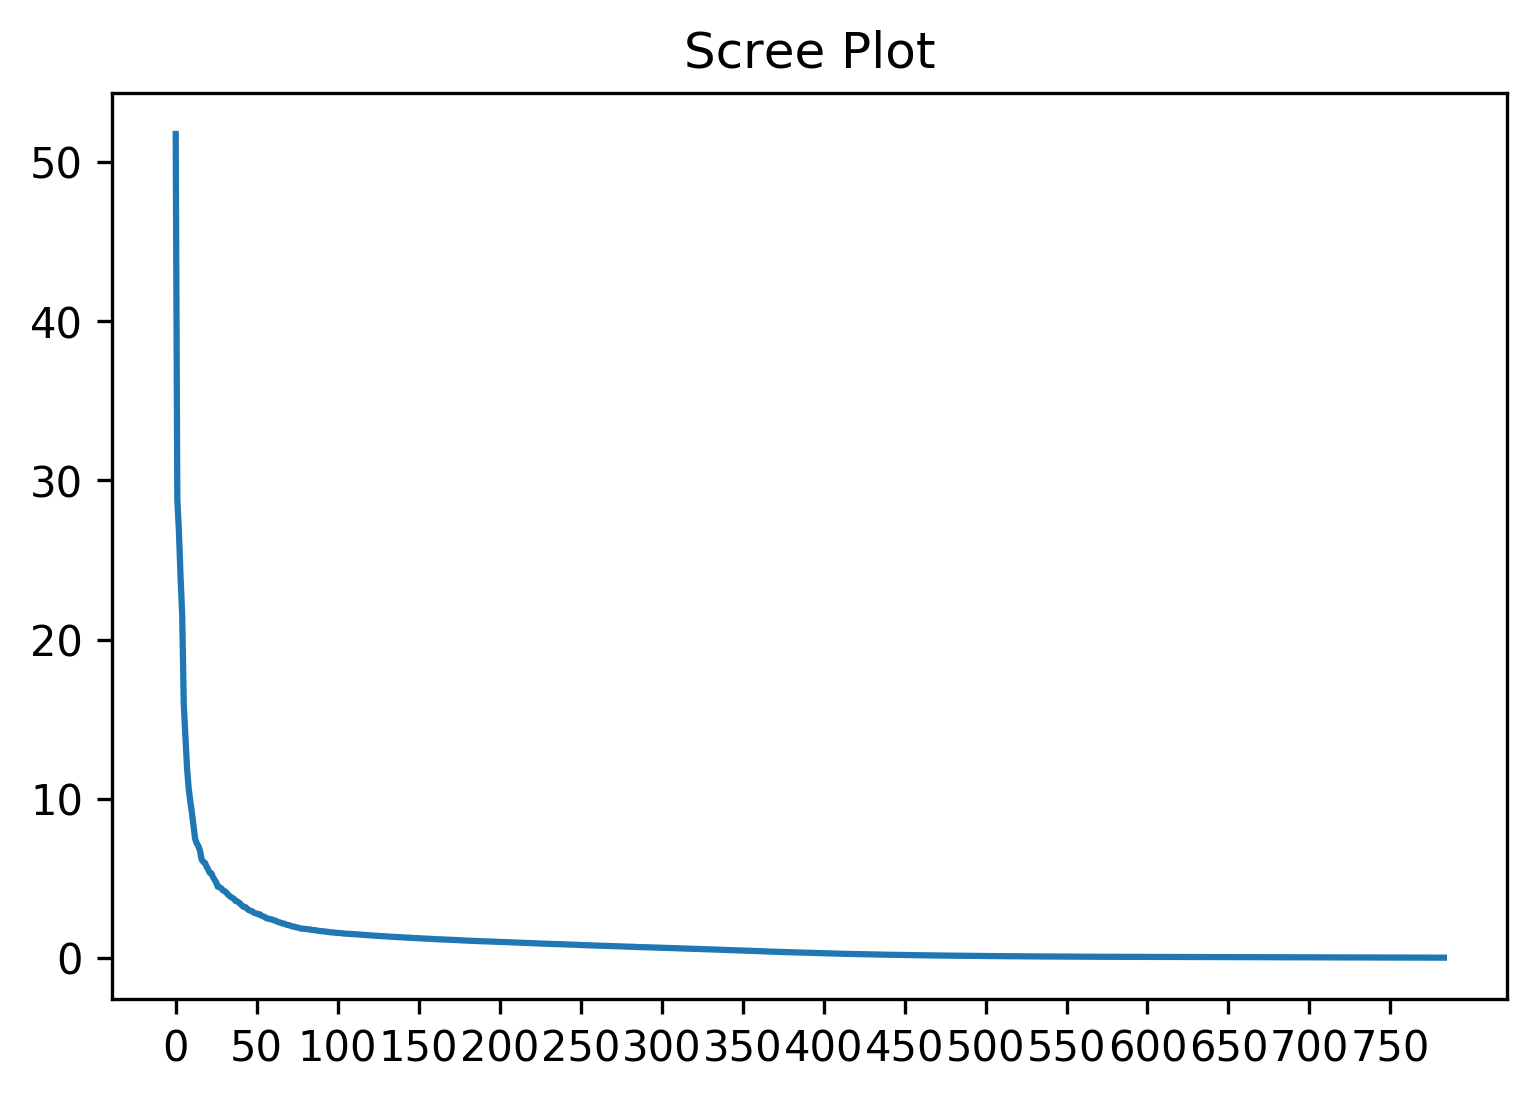
\includegraphics[width=14cm]{../plots/Q2_ScreePlot.png}
\end{center}
\noindent
According to the scree plot, the explained variance drops sharply from 0 to 50. A cut-off around 10 is good since after that, the amount of variance explained by the selected component is relatively small.\\\\
\textbf{Projected Data With Top 20 Eigenvalues in PCA}
\begin{center}
    \includegraphics[width=18cm]{../plots/Q2_PCATop19.png}
\end{center}
\noindent
We can see some clear separations between classes in the first 6 plots(PC1 vs PC2 to PC5 vs PC6). But after that almost all points are concentrated in the middle and we cannot tell them apart. Hence, keeping the first 6 components is a good choice. It is clearer to find the cut-off using pair plot since the slope is too large in the scree plot, making it difficult to find a specific cut-off value.\\\\
\textbf{PC1,2 Compared to PC5,6}
\begin{figure}[H]
\captionsetup[subfigure]{labelformat=empty}
\centering
\subfloat[]{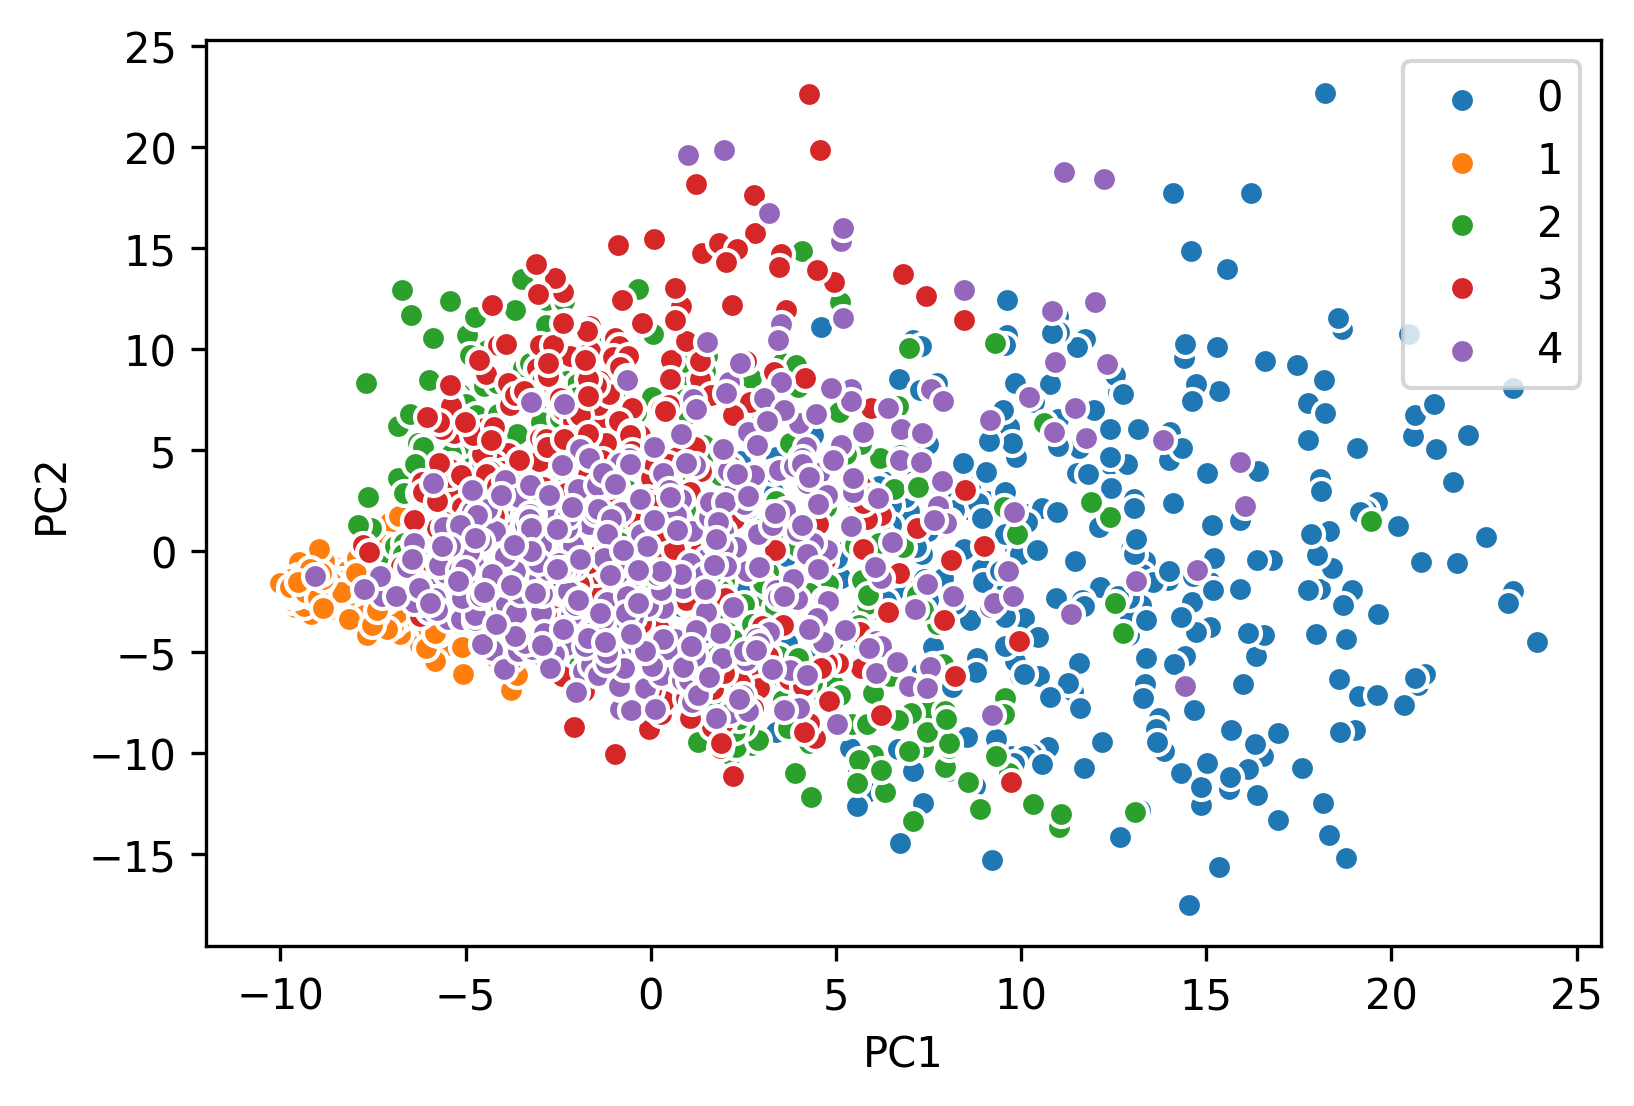
\includegraphics[width=0.48\textwidth]{../plots/Q2_PCA01.png}}
\subfloat[] {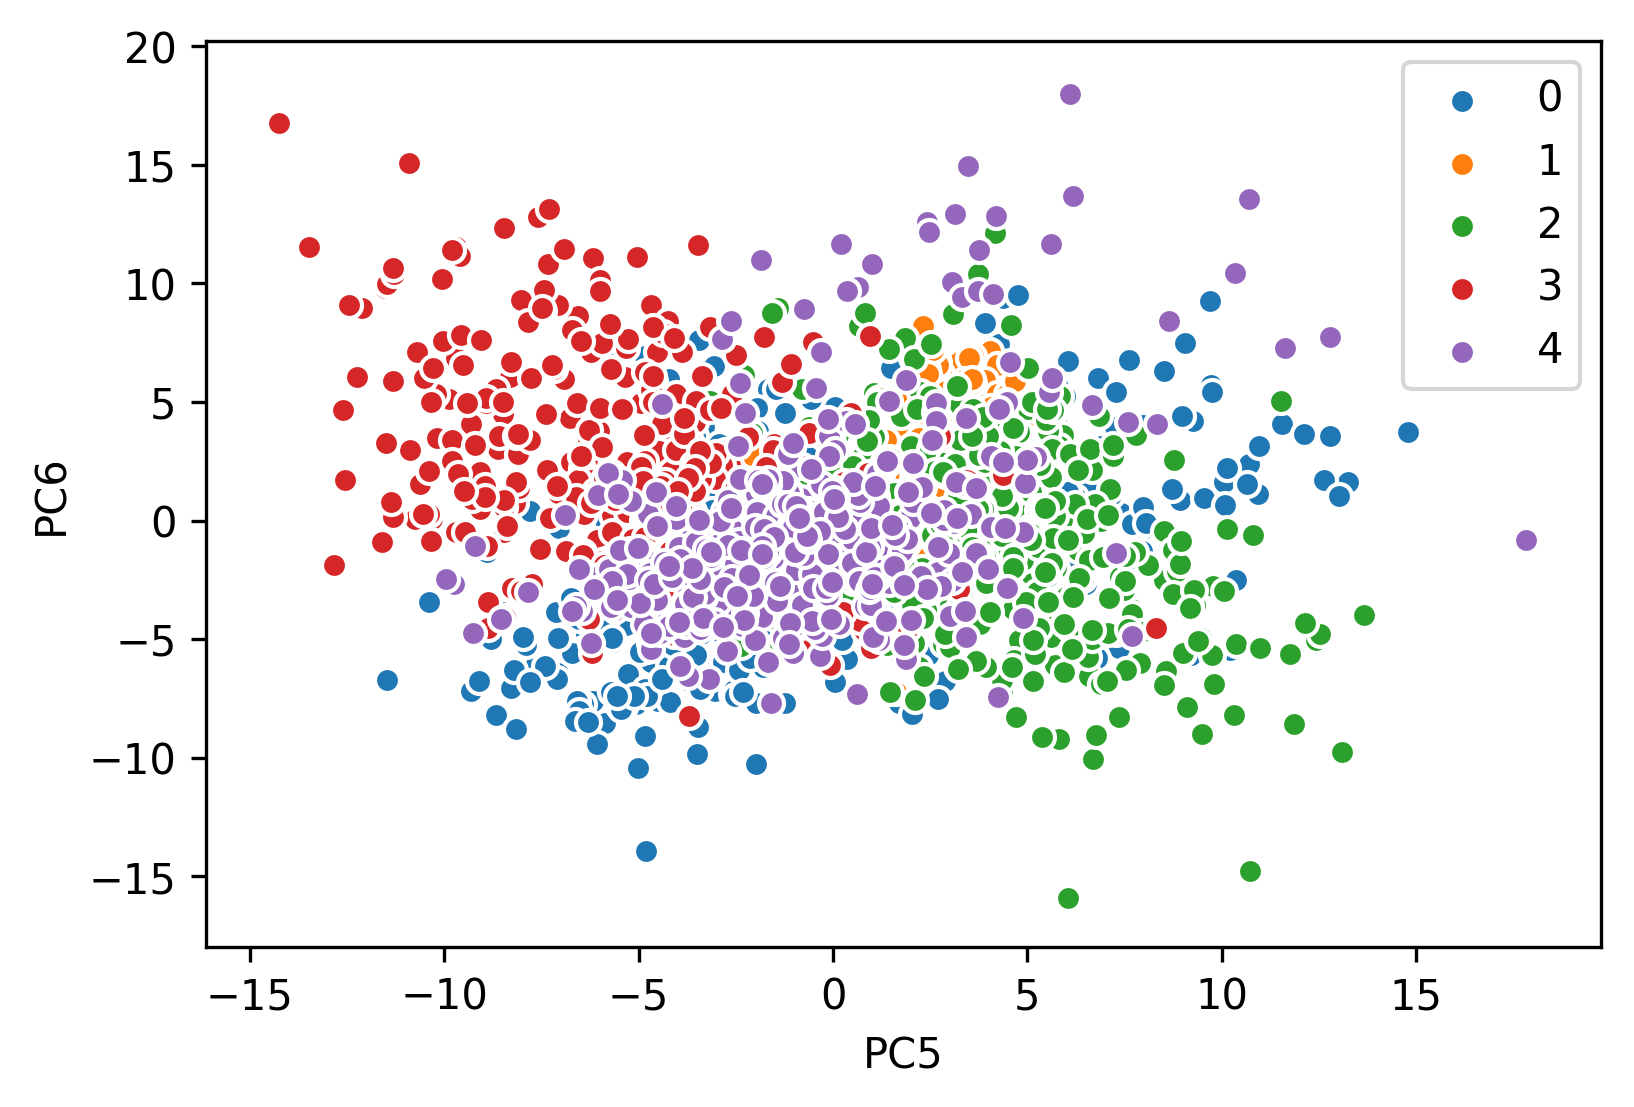
\includegraphics[width=0.48\textwidth]{../plots/Q2_PCA45.png}}
\end{figure}
\vspace*{-1.5cm}
\noindent
The first plot(PC1 vs PC2) mainly separates number 0 from other classes. It is difficult to distinguish the other 4 classes from the first plot as they all cluster on the left. Actually, PC2 does not help much to classify number 0, since the border between number 0 and others are almost vertical on the graph(PC1 = 10).\\
The second plot(PC5 vs PC6) makes some contribution to separating number 2 and number 3 from other classes. But it is not sufficient to use only PC5 and PC6 since there is large overlap in the middle between all numbers.\\
Although the first plot seems more orderless than the second plot, we can use it along to separate one class. But we cannot separate classes using only the second plot.\\\\
\textbf{SVD, PCA and Dual PCA Implementation}
\begin{spacing}{1.0}
\begin{lstlisting}
# Singular value decomposition
# input: an n*t array, n is the dimensionality and t is 
# the number of training examples
def svd_np(x):
    eigValueU, eigVectorU = np.linalg.eigh(np.dot(x, x.T))
    eigValueV, eigVectorV = np.linalg.eigh(np.dot(x.T, x))
    idxU = eigValueU.argsort()[::-1]
    idxV = eigValueV.argsort()[::-1]
    return eigVectorU[:,idxU], 
    np.sqrt(eigValueV[idxV] if x.shape[0] > x.shape[1] else eigValueU[idxU]), 
    eigVectorV[:,idxV].T
\end{lstlisting}
\begin{lstlisting}
# First get U, sigma and Vt from SVD
# s is a t*n array
U, sigma, Vt = svd_np(s.T)

# PCA
s.dot(U)

# Dual PCA
np.diag(sigma).dot(Vt[:s.shape[1],:]).T

# check if (sigma * Vt).T has the same result with build in PCA
print(np.allclose(np.absolute(np.diag(sigma).dot(Vt[:s.shape[1],:]).T), np.absolute(PCA().fit_transform(s))))
# True

# check if (U.T.dot(s.T)).T, which is s.dot(U), has the same result with build in PCA
print(np.allclose(np.absolute(s.dot(U)), np.absolute(PCA().fit_transform(s))))
# True
\end{lstlisting}
\end{spacing}
\noindent
Assume that we have already known the value of $U$, $\Sigma$ and $V^T$, run PCA and dual PCA 1000 times each and get the average runtime.\\
PCA: 22359.35 microseconds\\
Dual PCA: 22124.32 microseconds\\
Under this specific dataset, their performance is basically the same. In theory, dual PCA is only faster than PCA when the number of features $>>$ number of samples because maxtrix multiplication is simpler for Dual PCA under this condition.\\\\
\textbf{Prove that PCA is the best linear method for reconstruction}\\
Optimization problem: minimize the reconstruction error. $\stackunder{Minimize}{\textbf{U}}\norm{\overline{X}-UU^T\overline{X}}_F^2$ s.t. $U^TU=I$.
\begin{equation}
\begin{split}
\norm{\overline{X}-UU^T\overline{X}}_F^2 & = tr((\overline{X}-UU^T\overline{X})(\overline{X}-UU^T\overline{X})^T)\\
& = tr((\overline{X}-UU^T\overline{X})(\overline{X}^T-\overline{X}^TUU^T))\\
& = tr(\overline{X}\overline{X}^T) - 2tr(\overline{X}UU^T\overline{X}^T) + tr(\overline{X}UU^TUU^T\overline{X}^T)\\
& = tr(\overline{X}\overline{X}^T) - tr(\overline{X}UU^T\overline{X}^T)\\
& = tr(\overline{X}\overline{X}^T) - tr(U^T\overline{X}^T\overline{X}U)\\
& = const - tr(U^TSU)
\end{split}
\end{equation}
\noindent
The result indicates that minimizing the reconstruction error is equivalent to maximizing the trace of $U^TSU$, which is exactly what PCA is doing. Therefore, PCA is the best linear method for reconstruction.\\\\
\textbf{Projected Data With Top 4 Eigenvalues in LDA}
\vspace*{-1.0cm}
\begin{center}
    \includegraphics[width=18cm]{../plots/Q2_LDATop3.png}
\end{center}
\noindent
LDA1 separates number 0 and number 1. LDA2 separates number 4. LDA2 separates number 3 and LDA4 separates number 2.\\
Each LDA direction is mainly responsible for separating one or two classes, but that is not the case with each principle component.\\\\
\textbf{Compare LDA Optimization With PCA Optimization}\\
FDA optimization: $\stackunder{Maximize}{\textbf{U}}\;tr(U^TSU)$ s.t. $U^TS_WU=I$\\
PCA optimization: $\stackunder{Maximize}{\textbf{U}}\;tr(U^TSU)$ s.t. $U^TU=I$\\
FDA and PCA can be treated as the same optimization problem with different constraints. Since $S_W$ needs extra information(the label of the data), FDA is supervised linear transformation while PCA is unsupervised.\\
The ability of a component to separate different classes apart decreases as the number increases for both PCA and LDA becauese we sort the eigenvectors based on the magnitute of eigenvalues. Since the solution of FDA is the eigenvalues of $S_W^{-1}S_B$ and $S_B$ has rank $k-1$, where k is the number of classes, FDA only has $k-1$ solutions, therefore 3 subplots in LDA plot. On the LDA plot, we can see clearly the separation between classes along each LDA axis and the cohesion within each class because these are the optimization criteria of LDA. But we cannot see the same pattern in the PCA plot as PCA only maximize the overall variance on each PCA axis.
\end{document}